\documentclass[11pt]{article}
%\documentclass[11pt]{amsart}
\usepackage{geometry}                % See geometry.pdf to learn the layout options. There are lots.
\geometry{letterpaper}                   % ... or a4paper or a5paper or ... 
%\geometry{landscape}                % Activate for for rotated page geometry
\usepackage[parfill]{parskip}    % Activate to begin paragraphs with an empty line rather than an indent
\usepackage{hyperref}
\usepackage{graphicx}
\usepackage{amsmath,amssymb,latexsym}
\usepackage{epstopdf}
\DeclareGraphicsRule{.tif}{png}{.png}{`convert #1 `dirname #1`/`basename #1 .tif`.png}

\title{RIFIDI Engineering}
\author{James Percent \\ james@pramari.com}
\date{10/10/2010}                                           % Activate to display a given date or no date

\begin{document}
\maketitle

\tableofcontents
\listoffigures

%%%%%%%%%%%%%%%%%%%%%%%%%%%%%%%%%%%%%%%%%%%%%%%%%%%%%%%%%%%%%

\section{Introduction}

This document is the basis for the getting started on the RIFIDI engineering team.  It is the single source for all the information you need to get going.  It is obviously evolving, so let us know if you find anything missing, outdated, or incorrect.

Rather than litter the entire document with all the links, we have chosen a citation-based reference approach.  This keeps the presentation concise and the reference material co-located.   Citations should be clickable and any link within a citation should also be directly clickable.   This may seem annoying at first, but in the end we think having a concise index to the reference material is highly advantageous and worth a bit of clicking around.

%%%%%%%%%%%%%%%%%%%%%%%%%%%%%%%%%%%%%%%%%%%%%%%%%%%%%%%%%%%%%

\section{Operating System}\label{os}

This section provides information about installing and configuring Ubuntu Linux, which is our supported platform.  We should be able to run on any platform that supports Java 6, but such configurations are beyond the scope of this document.

The supported version of Ubuntu is 10.04.1 LTS, Lucid Lynx \cite{ubuntu, lucid}.  Instructions regarding Ubuntu installation and configuration can be found in \cite{lucid-doc}.  If you're not familiar with Ubuntu Linux, please take note of the package management system because it is an important piece of the platform in terms of getting your environment up and running.  An old tutorial is here \cite{apt-get-tut}, and, as always, Google is your friend.

The are only a few packages required to setup the environment; this command should work:
\begin{verbatim}
	$ sudo apt-get install eclipse emacs23 sun-java6-jdk thunderbird vim.
\end{verbatim}

Please note that, the period at the end of the command is a syntactic element of the English language, and it is not part of the command.

%%%%%%%%%%%%%%%%%%%%%%%%%%%%%%%%%%%%%%%%%%%%%%%%%%%%%%%%%%%%%

\section{Network and Email}

Our Pramari email accounts are our primary means of communication.  All email communication for company related information should happen via Pramari email accounts.   Our emails are proprietary and confidential and should be treated with care.  

Each user has a soft limit of 100 megabytes of email.  We recommend using the Mozilla Thunderbird email client \cite{thunderbird}.  If you completed Section~\ref{os}, then you already have Thunderbird installed.

Email can also be accessed through a web client \cite{webmail, harwood}; the server, $harwood.textdrive.com$ must be selected from the drop-down list.  Your userID is	 $firstname-pramari$; ask someone for your initial password.

The steps required to configure Thunderbird are straight forward: 
\begin{itemize}
\item add a new account; and
\item use the settings shown in Figures~\ref{fig:thunderbird1}-~\ref{fig:thunderbird3}, substituting your name and user-id for Prasith Govin and pgovin respectively.
\end{itemize} 

\begin{figure}
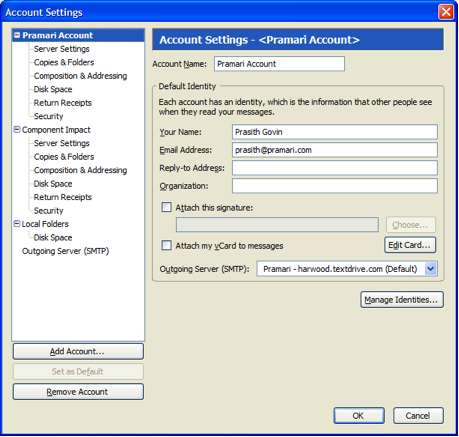
\includegraphics{thunderbird1.png}
\caption{\label{fig:thunderbird1} Pramari Account Settings}
\end{figure}

\begin{figure}
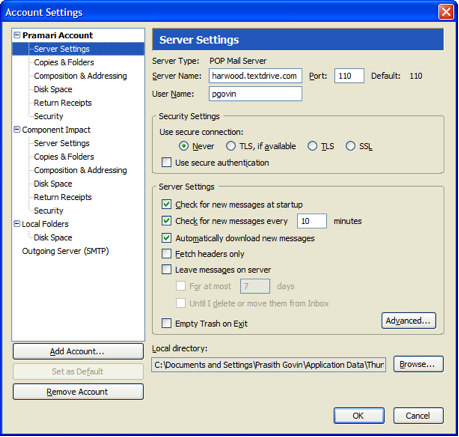
\includegraphics{thunderbird2.png}
\caption{\label{fig:thunderbird2} Server Settings}
\end{figure}

\begin{figure}
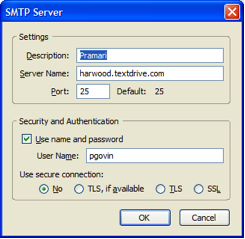
\includegraphics{thunderbird3.png}
\caption{\label{fig:thunderbird3} SMTP Settings}
\end{figure}

%%%%%%%%%%%%%%%%%%%%%%%%%%%%%%%%%%%%%%%%%%%%%%%%%%%%%%%%%%%%%

\section{Project Management Software}

We use Scrum to manage our development projects.  There's a plethora of Scrum tutorials, guides and books, but you can probably grok everything you need on-the-job.  That said, I recommend \cite{scrum-guide} as a brief introduction, and the original publication \cite{scrum-book} for a more thorough treatment.  We have a copy of \cite{scrum-book} in the office.

We use basecamp \cite{basecamp} for client-facing project management and documentation, and we use Rally \cite{rallydev} for Sprint planning and tracking (Sprints are the units of work in Scrum).  You should have accounts to both of these, so let someone know if you do not.

%%%%%%%%%%%%%%%%%%%%%%%%%%%%%%%%%%%%%%%%%%%%%%%%%%%%%%%%%%%%%

\section{Eclipse Setup}

Our development process, for better or worse, is very tightly coupled to the Eclipse platform \cite{eclipse}.  If you completed Section~\ref{os}, then Eclipse should be installed on your system.  From the Ubuntu desktop, click: \textit{Applications$\rightarrow$Development$\rightarrow$Eclipse}.   We recommend creating a workspace for each project, as depicted in Figure~\ref{fig:eclipse1}.

All RIFIDI-based software can be downloaded from our online repositories \cite{rep-edge, rep-external, rep-ambient}.  We use Subclipse \cite{subclipse} to interface with our SVN server.  To install Subclipse, from within Eclipse, click:
\textit{Help$\rightarrow$Install new software} as shown in Figure~\ref{fig:eclipse2}.  A dialog box will appear; click on add and paste in the Subclipse update site URL \cite{subclipse-update}; check all required boxes and click finish as shown in Figure~\ref{fig:eclipse3}.  Subclipse's documentation is installed with the plugin and can be accessed from Eclipse's help menu.  An online version can be found at \cite{subclipse-doc}.

We depend on several other packages: \textit{Eclipse Plug-in Development Environment, PDE/API Tools Environment, Java Development Tools, Eclipse XML Editors and Tools, JavaScript Developer Tools, Web, XML and Java EE Development}.  To install these packages, click: \textit{Help$\rightarrow$Install new software}.  From the drop-down box select the Galileo update site \cite{galileo} and select the packages as shown in Figure~\ref{fig:eclipse4}.

\begin{figure}
\resizebox{\textwidth}{!}{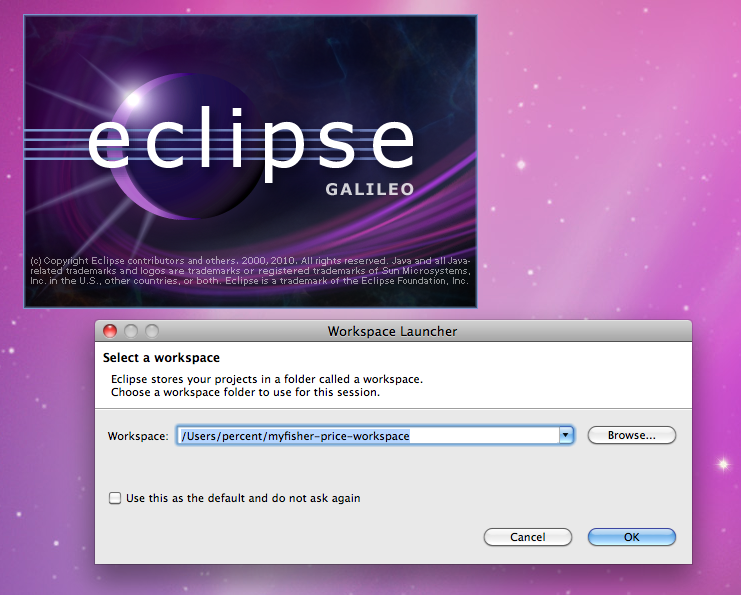
\includegraphics{eclipse1.png}}
\caption{\label{fig:eclipse1} Eclipse Workspace}
\end{figure}

\begin{figure}
\resizebox{\textwidth}{!}{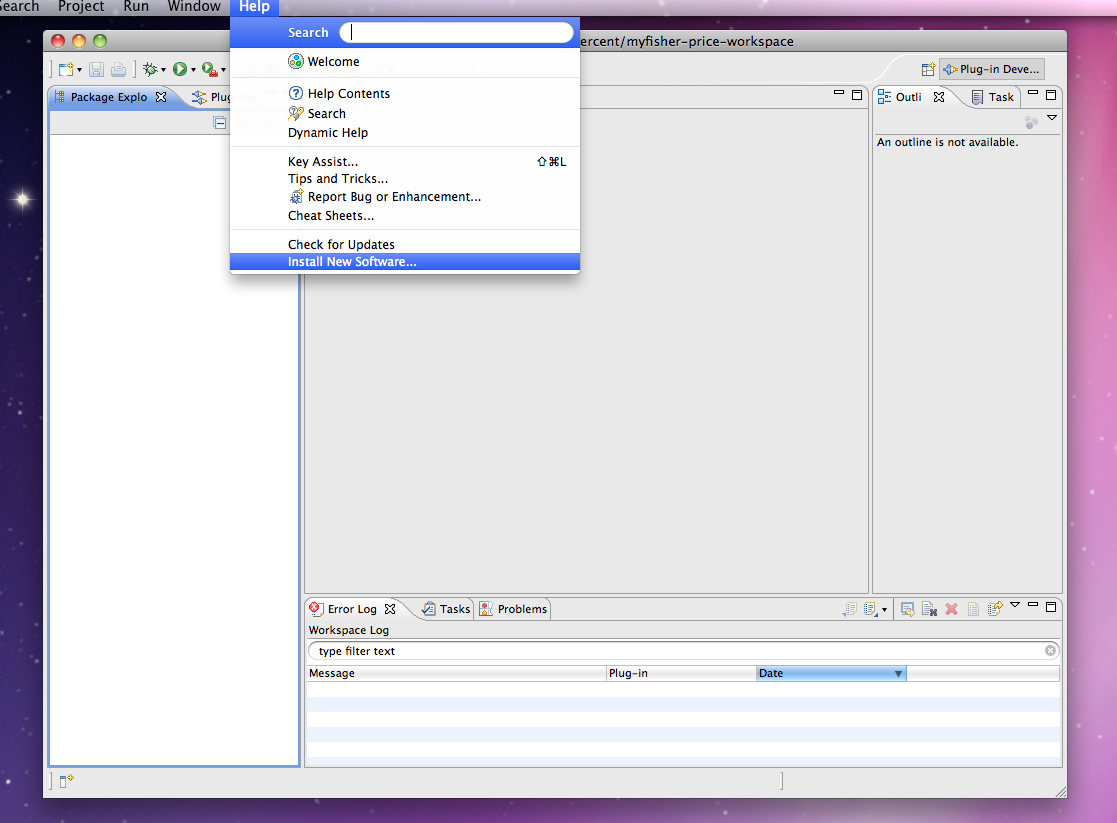
\includegraphics{eclipse2.png}}
\caption{\label{fig:eclipse2} Eclipse Software Installation }
\end{figure}

\begin{figure}
\resizebox{\textwidth}{!}{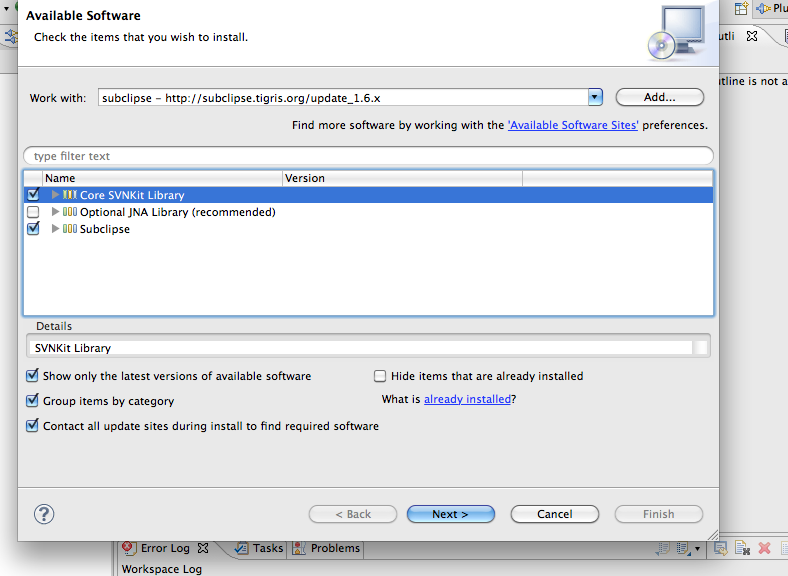
\includegraphics{eclipse3.png}}
\caption{\label{fig:eclipse3} Subclipse }
\end{figure}

\begin{figure}
\resizebox{\textwidth}{!}{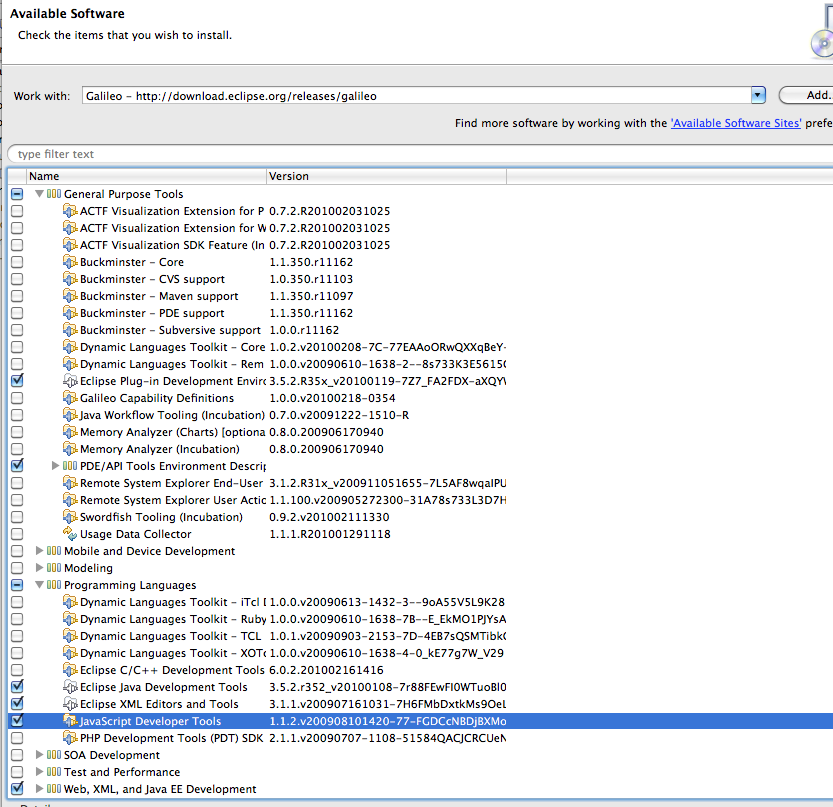
\includegraphics{eclipse4.png}}
\caption{\label{fig:eclipse4} Additional Eclipse Packages }
\end{figure}

%%%%%%%%%%%%%%%%%%%%%%%%%%%%%%%%%%%%%%%%%%%%%%%%%%%%%%%%%%%%%

\section{Edge Server}
 
 \subsection{Background}
 
The Edge Server is an OSGi-based service platform.  Our development is done within the Eclipse Plug-in Development Environment (PDE) \cite{pde}.  PDE provides OSGi tooling support and is based on Equinox \cite{equinox}, which is the reference implementation of the OSGi Alliance \cite{osgi}.

OSGi is essentially a dynamic module framework for Java.  The fundamental unit of decomposition in OSGi-based systems is the bundle; everything is encapsulated by a bundle.  

A bundle is basically a collection of packages and compile and run time dependancies.  Each bundle has a manifest file which is where these dependancies are specified.  The bundle's manifest file contains its unique identification, which includes its version, and specifies the packages it imports and exports.

The bundle lifecyle state-machine is depicted in Figure~\ref{fig:state}.  When the OSGi run-time is started every available bundle is installed.  If all the dependencies of a given bundle are met, then the bundle is resolved and it can be started.  A bundle must be stopped to be uninstalled or restarted.  Bundles are automatically stopped by the OSGi runtime when it is shutdown.

An essential part of developing PDE services is the target platform.  The target platform defines all the bundles that a PDE-based service can use.  Therefore, it contains all the OSGi bundles as well as any other third-party bundles that are used.   PDE provides a basic target platform, but the Edge Server extends it with many third-party bundles.  The target platform is well documented in the help chapter: \textit{Plug-in Development Environment Guide}.

Dependency injection \cite{di} is a design paradigm whereby the logic of the system is separated from acquiring and configuring dependancies.  The Edge Server relies on Spring Dynamic Modules \cite{spring-dm} to register services in the OSGi service registry and to handle dependency injection.  Each bundle has a Spring directory that defines its services and dependency injection rules.
 
\begin{figure}
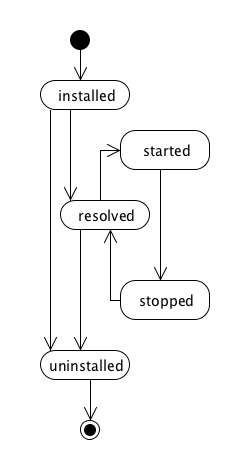
\includegraphics{lifecyle.png}
\caption{\label{fig:state} Lifecyle of a Bundle}
\end{figure}
 
 \subsection{Edge Server Configuration}
 
Now we are ready to checkout the Edge Server sources.  To accomplish this we need to switch to the SVN Repository Exploring perspective, as shown in Figures~\ref{fig:eclipse5} and \ref{fig:eclipse6}.  

Next, we need to add the Edge Server repository \cite{rep-edge}.  From within the SVN Repositories tab, right-click and select: \textit{New$\rightarrow$Repository Location} as shown in Figure~\ref{fig:eclipse7}.  A dialog-box will appear and the URL from \cite{rep-edge} needs to be pasted into it, as shown in Figure~\ref{fig:eclipse8}. 
 
 Next, we need to checkout the Edge Server sources.  From the Exploring perspective click: \textit{rifidi$\rightarrow$trunk}.  Select the following folders: \textit{org.rifidi.app.example, org.rifidi.app.template, org.rifidi.edge.api, org.rifidi.edge.app.diag, org.rifidi.edge.app.tracking, org.rifidi.edge.console, org.rifidi.edge.core, org.rifidi.edge.init and Rifidi-SDK}.  Subsequently right-click and select \textit{Checkout}.  Figure~\ref{fig:eclipse9} shows you what this looks like.  This takes about 10 - 30 minutes to complete depending on connection speeds.  Now would be a good time to grab some coffee.  

After the download completes, return to the Java perspective, so that we can set the target platform.  To set the target platform, from within the package explorer panel, open \textit{Rifidi-SDK$\rightarrow$RifidiHome$\rightarrow$org.rifidi.edge.target.target}.  This should come up in a special Eclipse target-platform-editor.  Click \textit{Set as Target Platform} as shown in Figure~\ref{fig:eclipse10}.
  
Finally we need to setup the run configuration.  We have included a EdgeServer.launch file in the Rifidi-SDK, so an Eclipse run-configuration already exists.  Open the run configuration as shown in Figure~\ref{fig:eclipse11}, and find the \textit{Edge Server} run configuration under \textit{OSGI Framework} as show in Figure~\ref{fig:eclipse12}, and click run.  To confirm the system is up and running, from the Eclipse console, type apps as shown in Figure~\ref{fig:eclipse13}.

\begin{figure}
\resizebox{\textwidth}{!}{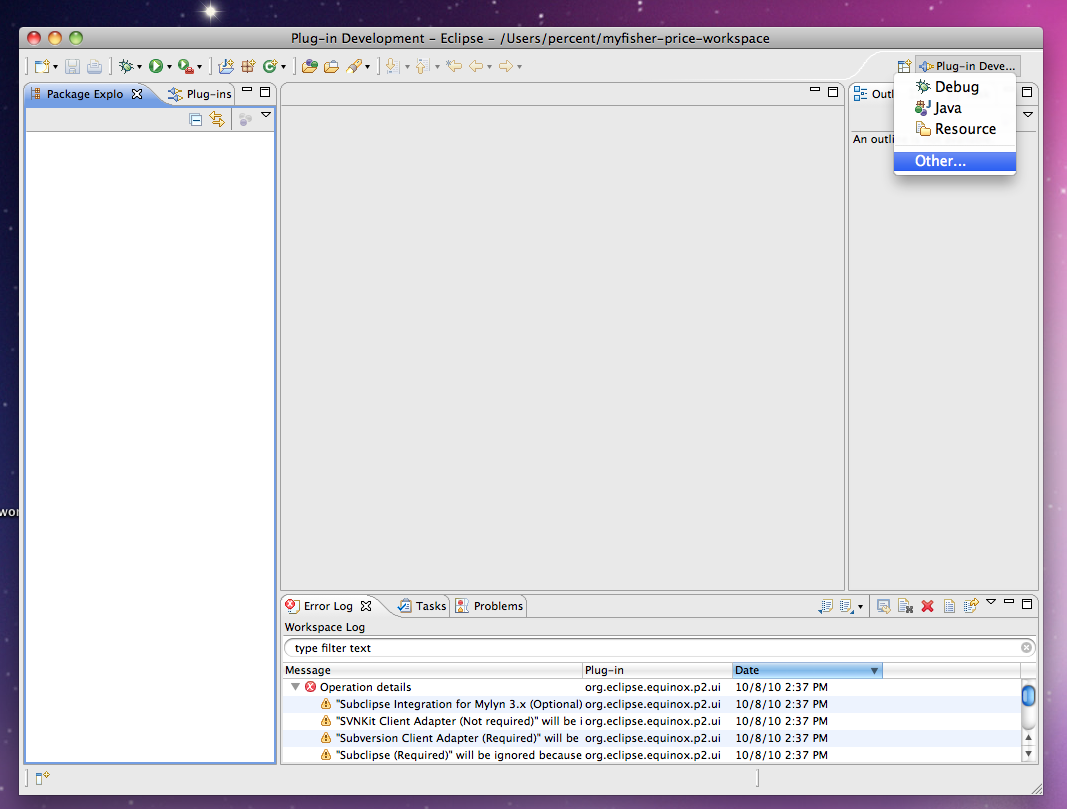
\includegraphics{eclipse5.png}}
\caption{\label{fig:eclipse5} Switching Perspective}
\end{figure}

\begin{figure}
\resizebox{\textwidth}{!}{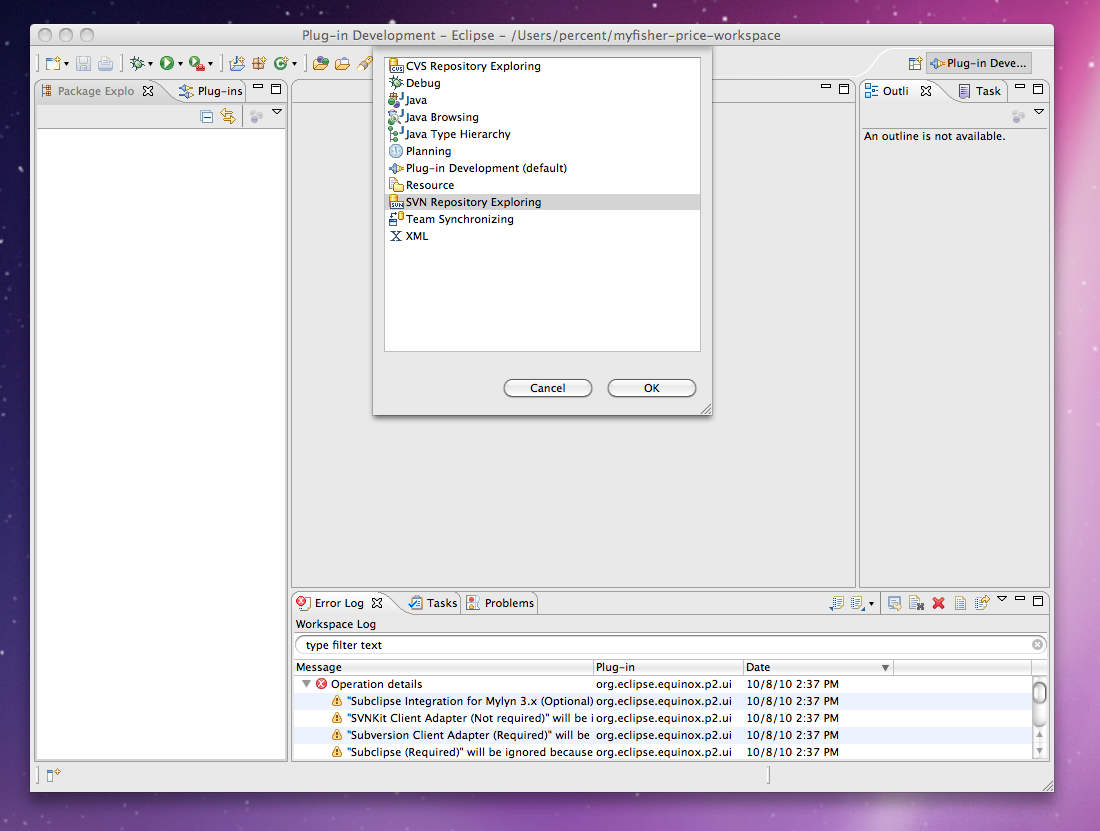
\includegraphics{eclipse6.png}}
\caption{\label{fig:eclipse6} SVN Exploring Perspective }
\end{figure}

 
\begin{figure}
\resizebox{\textwidth}{!}{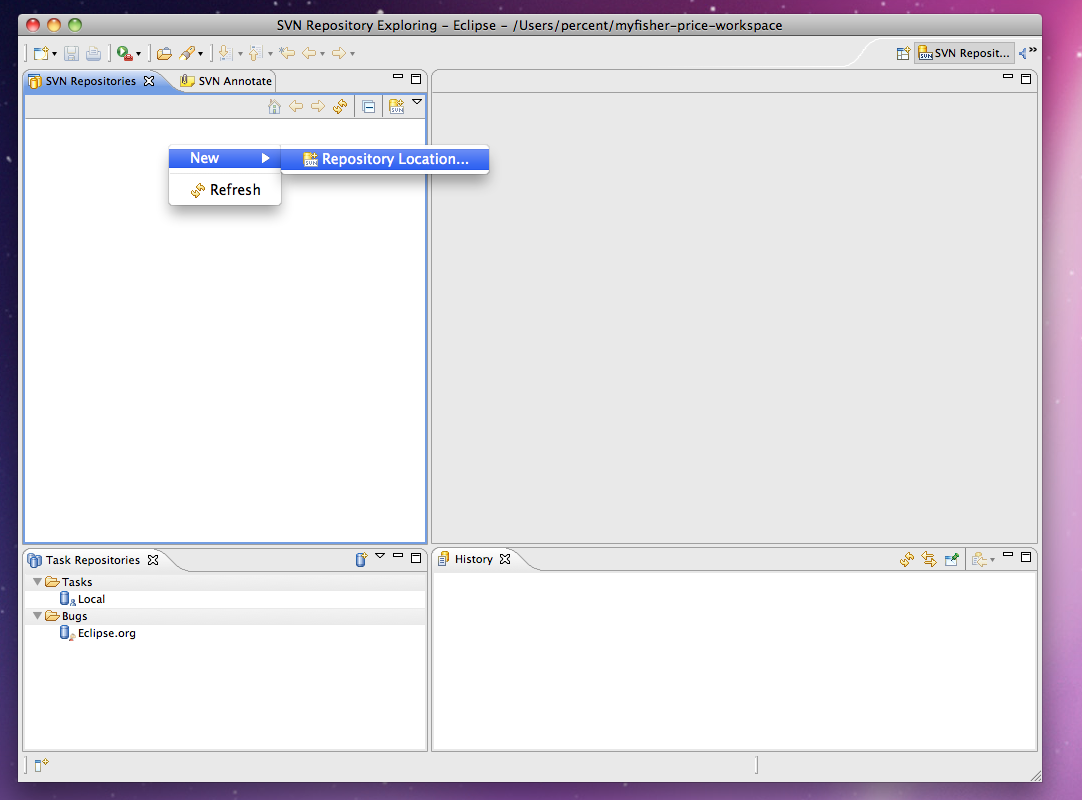
\includegraphics{eclipse7.png}}
\caption{\label{fig:eclipse7}Adding a New Repository 1}
\end{figure}


\begin{figure}
\resizebox{\textwidth}{!}{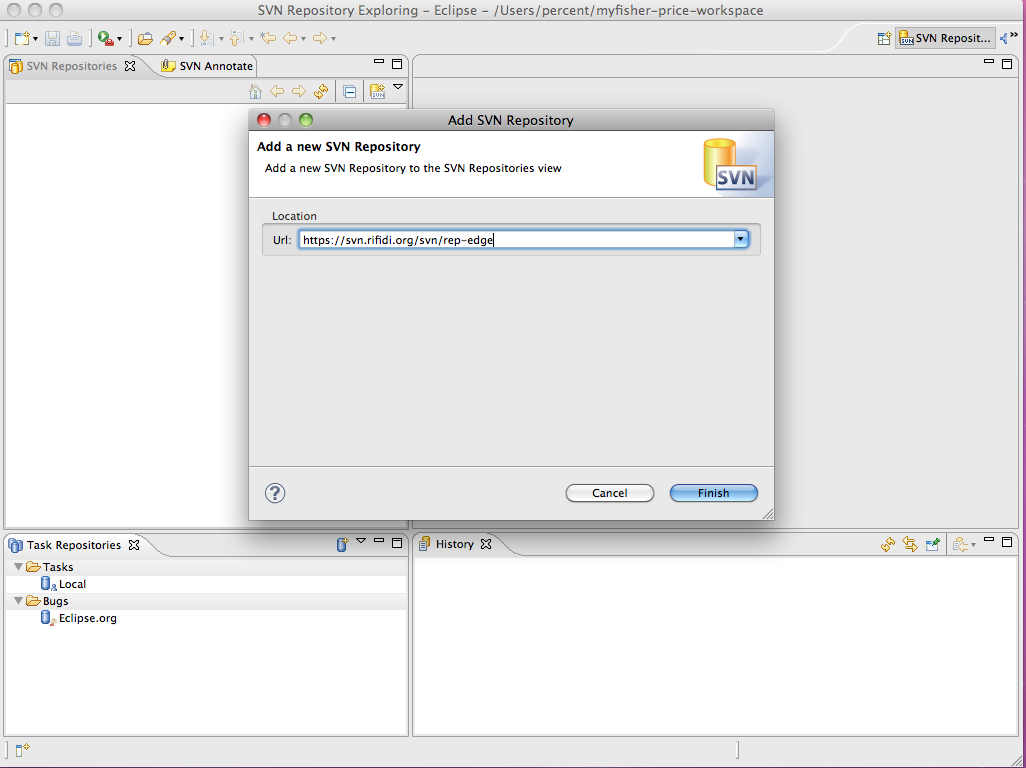
\includegraphics{eclipse8.png}}
\caption{\label{fig:eclipse8}  Adding a New Repository 2}
\end{figure}
 
 
\begin{figure}
\resizebox{\textwidth}{!}{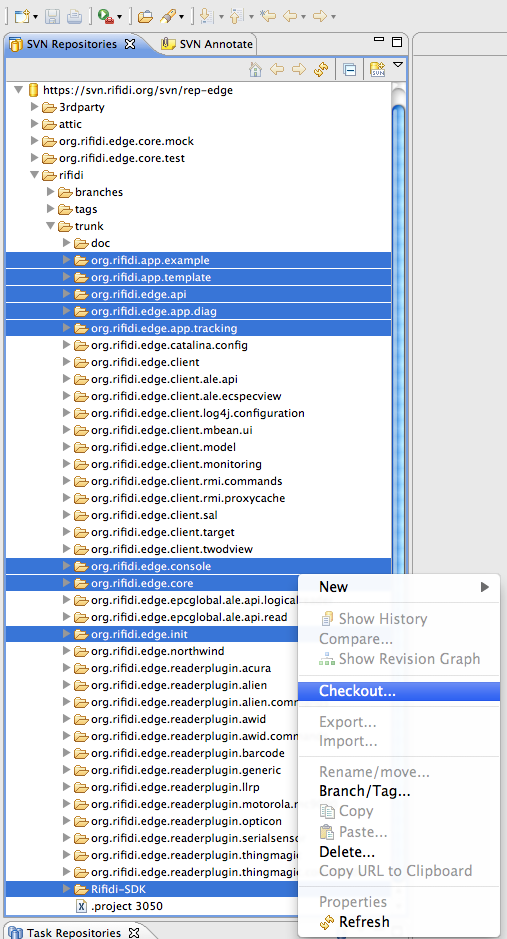
\includegraphics{eclipse9.png}}
\caption{\label{fig:eclipse9} Edge Server Source Checkout}
\end{figure}

\begin{figure}
\resizebox{\textwidth}{!}{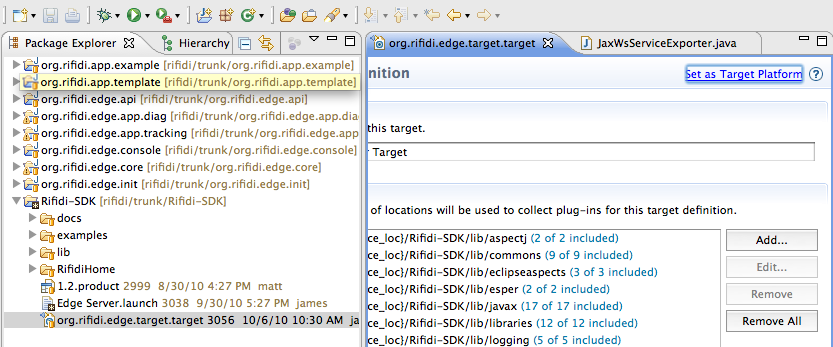
\includegraphics{eclipse10.png}}
\caption{\label{fig:eclipse10} Setting the Target Platform}
\end{figure}

\begin{figure}
\resizebox{\textwidth}{!}{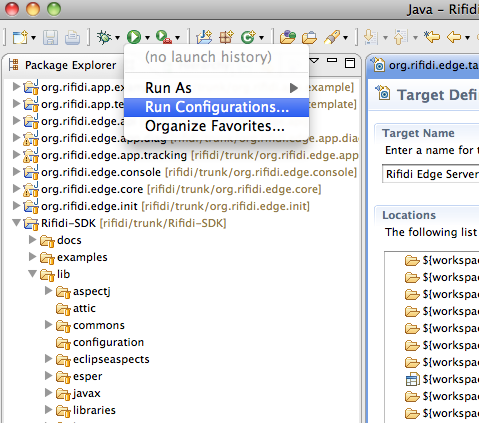
\includegraphics{eclipse11.png}}
\caption{\label{fig:eclipse11} Run Configurations}
\end{figure}

\begin{figure}
\resizebox{\textwidth}{!}{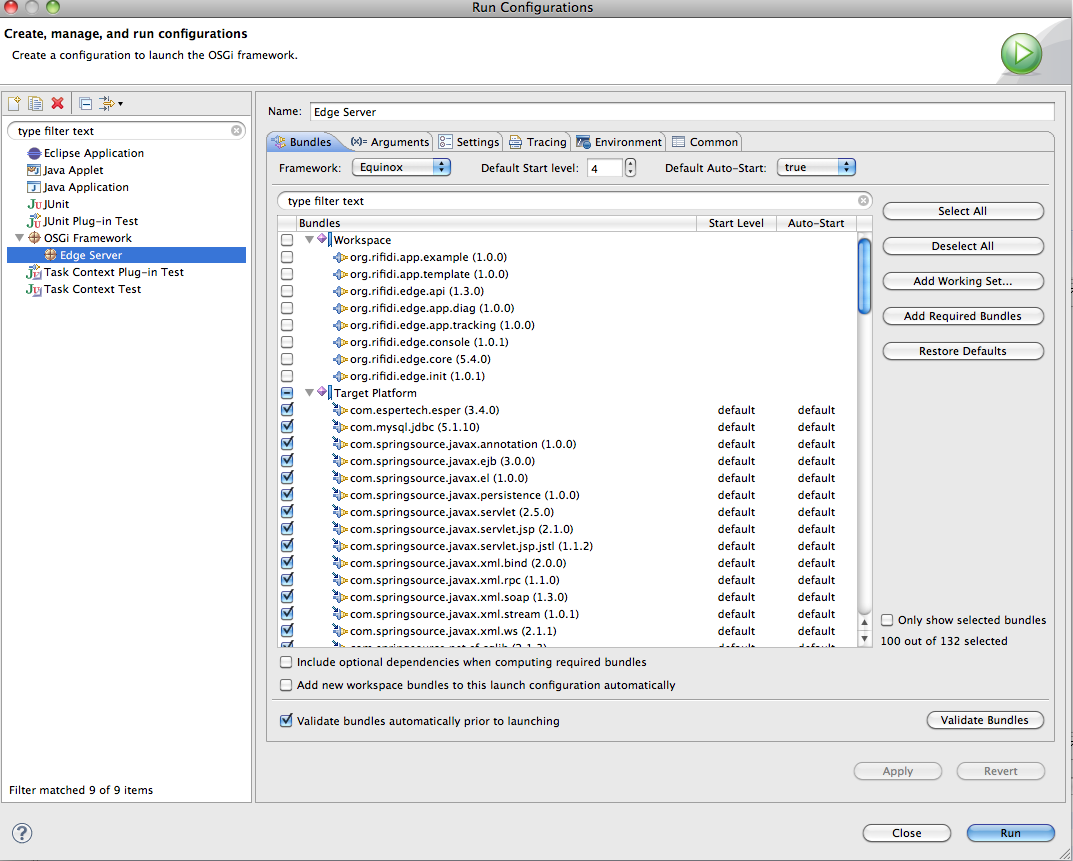
\includegraphics{eclipse12.png}}
\caption{\label{fig:eclipse12} Default Edge Server Run Configuration}
\end{figure}

\begin{figure}
\resizebox{\textwidth}{!}{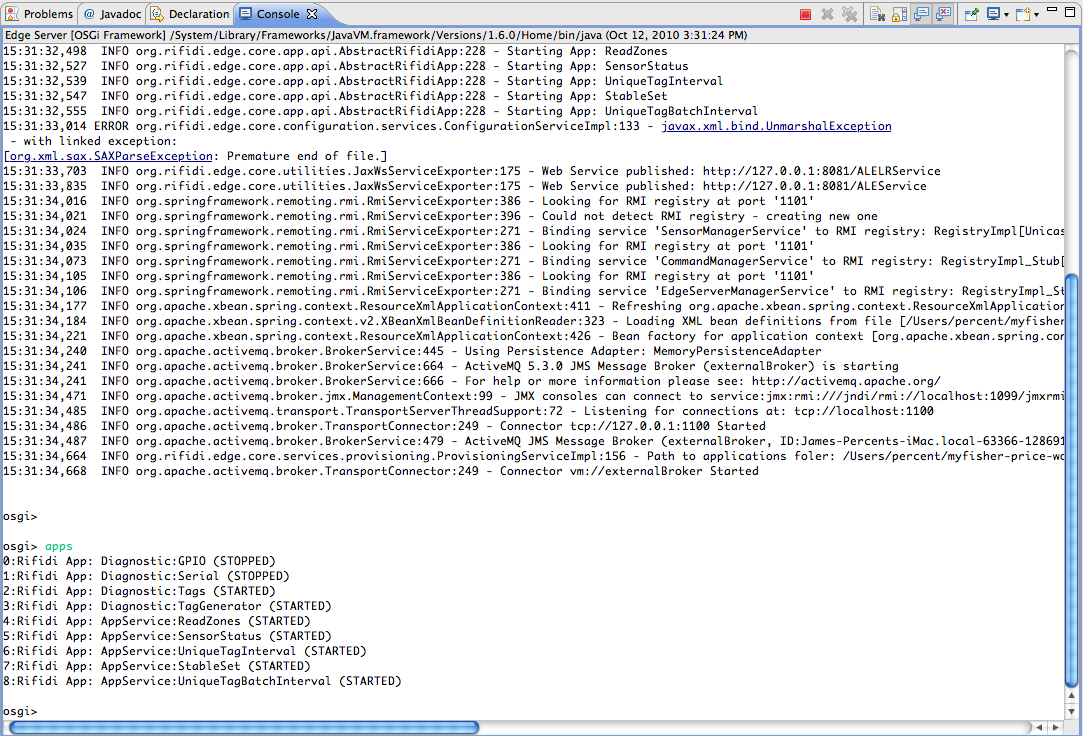
\includegraphics{eclipse13.png}}
\caption{\label{fig:eclipse13} OSGi Console}
\end{figure}

\subsection{Running Unit, System and RegressionTests}

%%%%%%%%%%%%%%%%%%%%%%%%%%%%%%%%%%%%%%%%%%%%%%%%%%%%%%%%%%%%%

\section{Developing Edge Server Applications}
\subsection{My Fisher-Price RIFIDI Application}
\subsection{Testing My Fisher-Price RIFIDI Application}

%%%%%%%%%%%%%%%%%%%%%%%%%%%%%%%%%%%%%%%%%%%%%%%%%%%%%%%%%%%%

\section{Modifying the Edge Server}
\subsection{Configuration}
\subsection{Deployment}

%%%%%%%%%%%%%%%%%%%%%%%%%%%%%%%%%%%%%%%%%%%%%%%%%%%%%%%%%%%%

\clearpage

\begin{thebibliography}{99}
\bibitem{ubuntu} Ubuntu Releases.  \url{http://releases.ubuntu.com}.
\bibitem{lucid} Ubuntu 10.04.1.  \url{http://releases.ubuntu.com/lucid}.
\bibitem{lucid-doc} Ubuntu 10.04.1 Documentation. \url{https://help.ubuntu.com/10.04/index.html}.
\bibitem{apt-get-tut} Apt.  \url{http://www.debian.org/doc/manuals/apt-howto/ch-apt-get.en.html}.
\bibitem{webmail}  Webmail.  \url{http://webmail.textdrivehosting.com/index.php}.
\bibitem{thunderbird} Thunderbird. \url{http://www.mozilla.org/projects/thunderbird}.
\bibitem{harwood} Mail server \url{harwood.textdrive.com}.
\bibitem{basecamp} Pramari Basecamp.  \url{https://pramari.basecamphq.com}.
\bibitem{rallydev}  Rally.  \url{https://community.rallydev.com}.
\bibitem{scrum-book}  Schwaber, Ken. Agile Project Management with Scrum.
\bibitem{scrum-guide} Scrum Guide.  \url{http://www.scrum.org/scrumguideenglish}. 
\bibitem{rep-edge} RIFIDI Edge Server. \url{https://svn.rifidi.org/svn/rep-edge}.
\bibitem{rep-external} RIFIDI Toolkit. \url{https://svn.rifidi.org/svn/rep-external}.
%\bibitem{rep-internal} RIFIDI ?? . \url{https://svn.rifidi.org/svn/rep-internal}.
\bibitem{rep-ambient} Ambient Project. \url{https://svn.rifidi.org/svn/rep-ambient}.
\bibitem{eclipse} Eclipse.  \url{http://www.eclipse.org.}.
\bibitem{pde} Plug-in Development Environment.  \url{http://www.eclipse.org/pde/}.
\bibitem{osgi-book} OSGI and Equinox: Creating Highly Modular Java� Systems.  \url{http://equinoxosgi.org}.
\bibitem{equinox} Equinox.  \url{http://www.eclipse.org/equinox}.
\bibitem{osgi} OSGi Alliance. \url{http://www.osgi.org/Main/HomePage}.	
\bibitem{spring-dm} Spring Dynamic Modules for OSGi Service Platforms.  \url{http://www.springsource.org/osgi}.
\bibitem{galileo} Eclipse Galileo.  \url{http://download.eclipse.org/releases/galileo}
\bibitem{subclipse} Subclipse.  \url{http://subclipse.tigris.org/}.
\bibitem{di} Fowler, M.  Dependency Injection.  \url{http://martinfowler.com/articles/injection.html}.
\bibitem{subclipse-doc} Subclipse online documentation.  \url{http://svn.collab.net/subclipse/help/index.jsp}.
\bibitem{subclipse-update} Subclipse.  \url{http://subclipse.tigris.org/update_1.6.x}.
\end{thebibliography}
\end{document}  


